\documentclass[letter,12pt]{article}
\usepackage[letterpaper,right=1.25in,left=1.25in,top=1in,bottom=1in]{geometry}
\usepackage{setspace}

\usepackage[utf8]{inputenc}   % allows input of special characters from keyboard (input encoding)
\usepackage[T1]{fontenc}      % what fonts to use when printing characters       (output encoding)
\usepackage{amsmath}          % facilitates writing math formulas and improves the typographical quality of their output
\usepackage[hyphens]{url}     % adds line breaks to long urls
\renewcommand{\UrlFont}{\ttfamily\small} % shrinks url font 1 step down
\usepackage[pdftex]{graphicx} % enhanced support for graphics
\usepackage{tikz}             % Easier syntax to draw pgf files (invokes pgf automatically)
\usetikzlibrary{arrows}

\usepackage{mathptmx}           % set font type to Times
\usepackage[scaled=.90]{helvet} % set font type to Times (Helvetica for some special characters)
\usepackage{courier}            % set font type to Times (Courier for other special characters)

\usepackage{rotating}         % sideway tables and figures that take a full page
\usepackage{caption}          % allows multipage figures and tables with same caption (\ContinuedFloat)

\usepackage{dcolumn}          % needed for apsrtable and stargazer tables from R to compile
\usepackage{arydshln}         % dashed lines in tables (hdashline, cdashline{3-4}, 
                              %see http://tex.stackexchange.com/questions/20140/can-a-table-include-a-horizontal-dashed-line)
                              % must be loaded AFTER dcolumn, 
                              %see http://tex.stackexchange.com/questions/12672/which-tabular-packages-do-which-tasks-and-which-packages-conflict

\usepackage{amssymb}          % has nicer empty set \varnothing, among much much more

%FOR SPANISH FORMATTING (HYPHENATION ETC.)
%% \usepackage[spanish]{babel}
%% \addto\captionsspanish{\renewcommand{\figurename}{Diagrama}} % cambia Figura por Diagrama

\usepackage[longnamesfirst, sort]{natbib}\bibpunct[]{(}{)}{,}{a}{}{;} % handles biblio and references 
%% \AtBeginDocument{\renewcommand\harvardand{y}} % change 'author and author' by Spanish 'author y author'

\newcommand{\mc}{\multicolumn}

%% TO ADD NOTES IN TEXT, PUT % BEFORE THE ONE YOU WANT DISBALED
%\usepackage[disable]{todonotes}                            % notes not showed
\usepackage[colorinlistoftodos, textsize=small]{todonotes} % show notes
\newcommand{\eric}[1]{\todo[color=red!15, inline]{\textbf{Eric:} #1}}
\newcommand{\alex}[1]{\todo[color=green!15, inline]{\textbf{Alejandro:} #1}}

% Format epigraph
\usepackage{epigraph}
\setlength\epigraphwidth{.8\textwidth}
\setlength\epigraphrule{0pt} % no rule

% multicolumns in appendix
\usepackage{multicol}

% change text color
\usepackage{xcolor}

\begin{document}

% \title{The removal of single-term limits, redistricting, and name recognition in Coahuila's state races}
% \title{Redistricting and the separation of incumbency and campaign effects: name recognition in Coahuila}
\title{The Personal Vote in Mexico: \\ Tables and Figures}
% \author{Eric Magar  \\ ITAM \\ \url{emagar@itam.mx} \and
%         Alejandro Moreno \\ ITAM \\ \url{amoreno@itam.mx} 
% }
\date{\today}
\maketitle

% \begin{center} \textbf{$\rightarrow$~~Preliminary draft~~$\leftarrow$} \\ (please inquire for new version)  \end{center}

\singlespacing

\begin{table}[h]
  \centering
%  \begin{tabular}{lccc}
%  \begin{tabular}{p{.25\textwidth} p{.18\textwidth} p{.18\textwidth} p{.18\textwidth}}
  \begin{tabular}{lccc}
%           & \mc{3}{c}{Incumbents and reelection} \\ [-.5ex]
%           & seek & succeed & return \\ \hline
                             & \mc{3}{c}{Incumbents (\%) who} \\ 
                             & sought      &             &            \\ [-.5ex]
                             & reelection  & reelected   & returned   \\ [-.5ex]
    Case                     &   ($a$)     &   ($b$)     & ($c=a\times b/100$) \\ \hline \\ [-1.25ex] 
    United States 1990--2010 &    91       &     94      &     86     \\ 
    Chile 1993--2000         &    71       &     83      &     59     \\
    Brazil 1994--2002        &    75       &     66      &     50     \\
    Uruguay 1985--1999       &    61       &     56      &     34     \\
    Colombia 1994--2002      &    53       &     65      &     34     \\                 
    Mexico 2021-2024         &    47       &     72      &     34     \\
    Argentina 1983--2001     &    25       &     76      &     19     \\ \\ [-1.25ex] \hline
  \end{tabular}
  \caption{The willing and the able to return to Congress in seven democracies. Column (a) reports the percentage of incumbents in the lower chamber that were renominated, column (b) the percentage of those renominated who won reelection for a consecutive term, and column (c) the return rate. Sources: \citet[][:658]{jones.etal.amateurLegis.2002} for Argentina; \citet{botero.renno-Career-reelec-br-col2007} for Brazil and Colombia; \citet{naviaIncumbency.2000} for Chile; \protect\url{https://emagar.github.io/2021-06-25-reeleccion-dipfed-6-jun.html} for Mexico (single-member-district deputies only); \citet{altman-chasquetti-Career-reelec-urug2005} for Uruguay; \protect\url{https://www.opensecrets.org/overview/reelect.php} for the U.S.}\label{T:retRate}
\end{table}

\newpage

\begin{table}[h]
  \centering
  \begin{tabular}{lc}
    Year &  \% returned  \\ \hline \\ [-1.25ex]
    1916 (Constitutional Congress) &          --- \\
    1917 &           18 \\
    1918 &           25 \\
    1920 &           15 \\
    1922 &           26 \\
    1924 &           25 \\
    1926 &           30 \\
    1928 &           40 \\
    1930 (Congress size nearly halved) &           42 \\
    1932 &           27 \\
    1934 (single-term limits effective) &            0 \\ [-1.25ex] \\ \hline
  \end{tabular}
  \caption{Reelection in the post-Revolutionary Chamber of Deputies up to 1934. Source: \citet{godoy.reeleccion.2014}.}\label{T:1920s}
\end{table}

\newpage

\begin{figure}[h]
  \centering
    \usetikzlibrary{calc}
    \begin{tikzpicture}
      \draw (0,0)  ellipse (3 and 2);
      \node[sloped,above] at ($(0,0)+(90:3 and 2)$) {\textsc{father}};
      \draw (3,0) ellipse (3 and 2);
      \node[sloped,above] at ($(3,0)+(90:3 and 2)$) {\textsc{son}};
      \draw (-3.5,-3) rectangle (6.5,3);
      \node [text width=2cm, text centered] at (-1.25,0)   {$l=$ land lost};
      \node [text width=2cm, text centered] at (4.25,0)    {$g=$ land gained};
      \node [text width=2cm, text centered] at (1.5,0)     {$r=$ land retained};
      \node at (1.5,-2.5) {$n=$ no man's land};
    \end{tikzpicture}
    \caption{Four clear and distinct lands arise from redistricting. \textsc{Father} and \textsc{son} represent 2014 and 2017 map districts, respectively.}\label{F:venn}
\end{figure}

\newpage

\begin{table}[h]
  \centering
\scalebox{.8}{
\begin{tabular}{llrccc}
 Son district               &  Father district            &       &                             & Revealed        & \\ [-.5ex]
 (2017)                     &  (2014)                     &  $S$  & Incumbent deputy            & ambition        & Margin \\ \hline
\\ [-1.2ex]
 \textsc{xii}-Ramos Arizpe  & \textsc{v}-Ramos Arizpe     & 1.000 & Lily Gutiérrez Burciaga     & \textbf{static} & $+14$ \\
 \textsc{i}-Acuña           & \textsc{xv}-Acuña           &  .798 & Gina Cano Torralva          & \textbf{static} & $-17$ \\ 
 \textsc{ii}-Piedras Negras & \textsc{xvi}-Piedras Negras &  .791 & Sonia Villarreal Pérez      & progressive     & $+12$ \\ 
 \textsc{x}-Matamoros       & \textsc{vii}-Torreón        &  .705 & Shamir Fernández Hernández  & none            & \\ 
 \textsc{xiv}-Saltillo      & \textsc{i}-Saltillo         &  .700 & Javier Díaz González        & \textbf{static} & $-12$ \\ 
 \textsc{ix}-Torreón        & \textsc{viii}-Torreón       &  .650 & Irma Castaño Orozco         & none            & \\ 
 \textsc{vii}-Matamoros     & \textsc{vi}-Torreón         &  .618 & Verónica Martínez García    & none            & \\ 
 \textsc{xvi}-Saltillo      & \textsc{ii}-Saltillo        &  .553 & Francisco Tobías Hernández  & none            & \\ 
 \textsc{iii}-Sabinas       & \textsc{xiii}-Múzquiz       &  .551 & Antonio Nerio Maltos        & none            & \\ 
 \textsc{xiii}-Saltillo     & \textsc{iv}-Saltillo        &  .459 & Martha Garay Cadena         & none            & \\ 
 \textsc{iv}-San Pedro      & \textsc{x}-San Pedro        &  .444 & Ana Isabel Durán Piña       & progressive     & $+3$ \\ 
 \textsc{v}-Monclova        & \textsc{xii}-Monclova       &  .408 & Melchor Sánchez de la Fuente& none            & \\ 
 \textsc{vi}-Frontera       & \textsc{xi}-Frontera        &  .377 & Lencho Siller Linaje        & progressive     & $+8$ \\ 
 \textsc{xiii}-Saltillo     & \textsc{iii}-Saltillo       &  .236 & José María Frausto Siller   & none            & \\ 
 \textsc{ix}-Torreón        & \textsc{ix}-Torreón         &  .204 & Luis Gurza Jaidar           & none            & \\ 
 \textsc{iii}-Sabinas       & \textsc{xiv}-Sabinas        &  .197 & Martha Morales Iribarrén    & none            & \\ 
 \\ [-1.2ex] \hline
\end{tabular}
}
\caption{District similarity index $S$ in the state of Coahuila. Mexican legislative districts rely on Roman numerals for identification, hyphenated in the Table with the district's administrative seat (\emph{cabecera distrital}.) All members were from the PRI (opposition deputies entered via proportional representation only). The margin is the percentage difference between the winner and runner-up in the subsequent race, positive if the incumbent won, negative otherwise.}\label{T:dsi}
\end{table}

\newpage

\begin{table}[h]
  \centering
  \begin{tabular}{cccc}
      & Campaign & Incumbency &  Total   \\ [-.5ex]
      & effect   & effect     &  effect  \\ \hline
    \\ [-1.2ex]
    1 & $r=g$    & $r>g$      &  $r>g$   \\
    2 & $r>l$    & $r=l$      &  $r>l$   \\
    3 & $r>n$    & $r>n$      &  $r>n$   \\
    4 & $l<g$    & $l>g$      &  $l~?~g$ \\ % \overset{?}{>}
    5 & $l=n$    & $l>n$      &  $l>n$   \\
    6 & $g>n$    & $g>n$      &  $g>n$   \\ \\ [-1.2ex] \hline 
  \end{tabular}
  \caption{Incumbency and campaign effects in name recognition hypotheses. Cells give expected relations in name recognition in the areas defined in Figure \ref{F:venn}. Thus, row 1 indicates that incumbency causes higher name recognition among voters in land retained than among voters in land gained, a difference not caused by the campaign effect; combining them gives the reported total effect.}\label{T:hyps}
\end{table}

\newpage

\begin{table}[h]
% % geog mean DV
% > # l   > # r   # g   # n   
% 0.214 & 0.304 & --- & 0.067 
% ---   & 0.393 & --- & 0.058 
% ---   & 0.729 & --- & 0.037 
% 0.167 & 0.5   & --- & 0.049 
% ---   & 0.518 & --- & 0.057 
% 0.143 & 0.738 & --- & 0.038 
% 0.033 & 0.095 & --- & ---   
% 0.064 & 0.048 & --- & ---   
% 0.040 & 0.405 & --- & ---   
  \centering
  \begin{tabular}{llrrrrrrr}
                & District/   &  \mc{4}{c}{Respondents}   & \mc{3}{c}{Mean $\texttt{recognize}$}  \\ 
    Incumbent   & municipio   &  $l$ & $r$ & $g$& $n$   & statewide & father & son  \\ \hline \\[-1.8ex] 
  %  \mc{9}{l}{~~A. \emph{Static ambition (SMD$\rightarrow$SMD)}} \\ \hdashline
    \mc{9}{l}{~~A. Static ambition} \\ \hdashline
  Javier Díaz González    & Saltillo    &  14 &  56 &  0  & 938 &  0.082      &  0.286  & 0.304 \\
  Lily Gutiérrez Burciaga & R. Arispe   &   0 &  56 &  0  & 952 &  0.076      &  0.393  & 0.393 \\
  Gina Cano Torralva      & Acuña       &   0 &  70 &  0  & 938 &  0.085      &  0.729  & 0.729 \\
  \\[-1.8ex] 
  %  \mc{9}{l}{~~B. \emph{Progressive ambition (SMD$\rightarrow$municipio)}} \\ \hdashline
    \mc{9}{l}{~~B. Progressive ambition} \\ \hdashline
  Lencho Siller           & Frontera    &  42 &  28 &  0  & 938 &  0.066      &  0.300  & 0.500 \\
  Sonia Villarreal Pérez  & P. Negras   &   0 &  56 &  0  & 952 &  0.082      &  0.518  & 0.518 \\
  Ana Isabel Durán Piña   & San Pedro   &  14 &  42 &  0  & 952 &  0.068      &  0.589  & 0.738 \\ 
  % \\[-1.8ex]
  %   \mc{9}{l}{~~C. \emph{Progressive ambition (PR$\rightarrow$municipio)}} \\ \hdashline
  % Armando PAN   & Frontera    & 966 &  42 &  0  &   0 &  0.036      & 0.036   & 0.095 \\
  % Lariza PAN    & P. Negras   & 966 &  42 &  0  &   0 &  0.063      & 0.063   & 0.048 \\
  % Leonel PPC    & Matamoros   & 966 &  42 &  0  &   0 &  0.056      & 0.056   & 0.405 \\
  \\[-1.8ex] \hline
  \end{tabular}
  \caption{Incumbents and their terrain. Deputies with static ambition sought reelection to the state assembly. Deputies with progressive ambition sought election to a municipal government. Columns $l$, $r$, $g$, and $n$ report the number of respondents sampled (out of 1,008) in each terrain category. Dependent variable means are for all respondents (statewide), for respondents in the pre-redistricting constituency (father) only, and for respondents in the post-redistricting constituency (son) only.}\label{T:terrenos}
\end{table}

\newpage

\begin{table}[h]
\centering
  \begin{tabular}{lrrr}
                          & \multicolumn{3}{c}{Hypotheses} \\
                          & total & incumbency & incumbency \\ [-0.5ex] 
                          & effect& effect     & effect \\  [-0.5ex] 
                          & $r>n$ & $l>n$ & $r = l$ \\ [-0.5ex] 
  Member                  & \footnotesize{(one-tailed)} & \footnotesize{(one-tailed)} & \footnotesize{(two-tailed)} \\ \hline \\[-1.8ex]
  \multicolumn{4}{l}{\textbf{~~~Static ambition}} \\
1 Javier Díaz González    & \color{green}{$<.001$} & \color{green}{$.029$} & \color{green}{$.442$} \\
2 Lily Gutiérrez Burciaga & \color{green}{$<.001$} & ---    & --- \\
3 Gina Cano Torralva      & \color{green}{$<.001$} & ---    & --- \\ \\[-1.8ex]
  \multicolumn{4}{l}{\textbf{~~~Progressive ambition}} \\
4 Lencho Siller           & \color{green}{$<.001$} & \color{green}{$.003$} & \color{red}{$.002$} \\
5 Sonia Villarreal Pérez  & \color{green}{$<.001$} & ---    & --- \\
6 Ana Isabel Durán Piña   & \color{green}{$<.001$} & \color{green}{$.036$} & \color{red}{$<.001$} \\
%   \multicolumn{4}{l}{\textbf{~~~PR, progressive ambition}} \\
% 7 Armando Pruneda Valdez  & \color{green}{$.030$}  & ---    & --- \\
% 8 Lariza Montiel Luis     & \color{red}{$.385$}    & ---    & --- \\
% 9 Leonel Contreras Pámanes& \color{green}{$<.001$} & ---    & --- \\
\\[-1.8ex] \hline
\end{tabular}
\caption{Hypothesis tests. Cells report p-values. Columns 1 and 2 respectively test that coefficients for $\texttt{retained}$ and $\texttt{lost}$ are positive, column 3 that $\texttt{retained}$'s coefficient equals $\texttt{lost}$'s (a likelihood-ratio test). Green indicates statistical evidence for incumbency effects, red lack thereof---note that column 3's incumbency hypothesis involves equality, so the aim here is to \emph{not} reject.}\label{T:hyp-tests}
\end{table}

\newpage

\begin{figure}[h]
  \centering
  \begin{tabular}{cc}
    Static ambition & Progressive ambition \\ \hline
    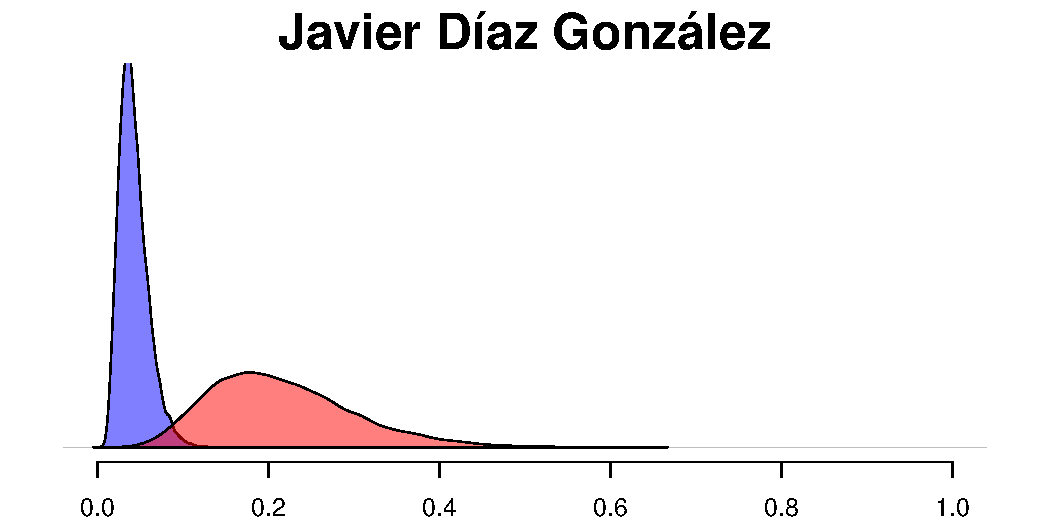
\includegraphics[width=.45\columnwidth]{../graphs/prReconoce1.pdf} &
    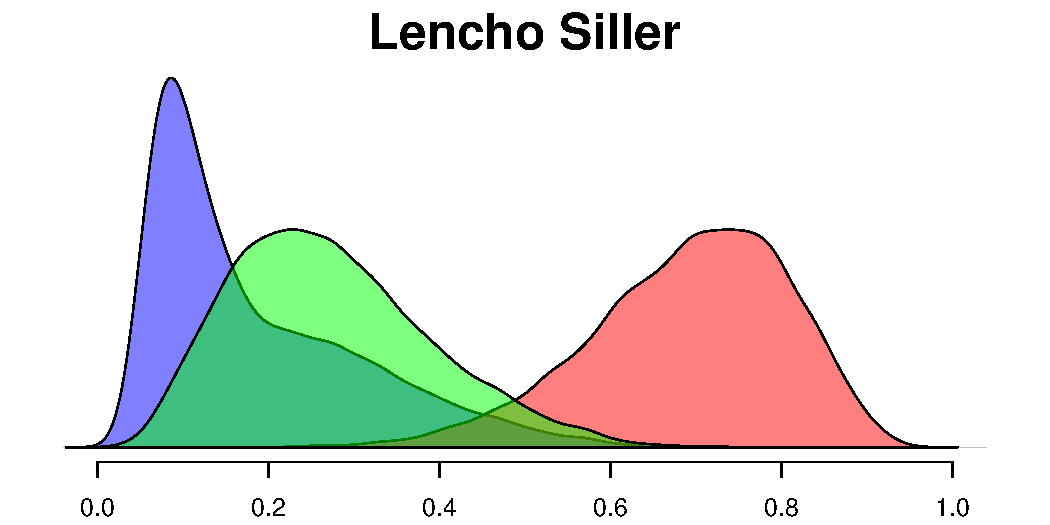
\includegraphics[width=.45\columnwidth]{../graphs/prReconoce6.pdf} \\
    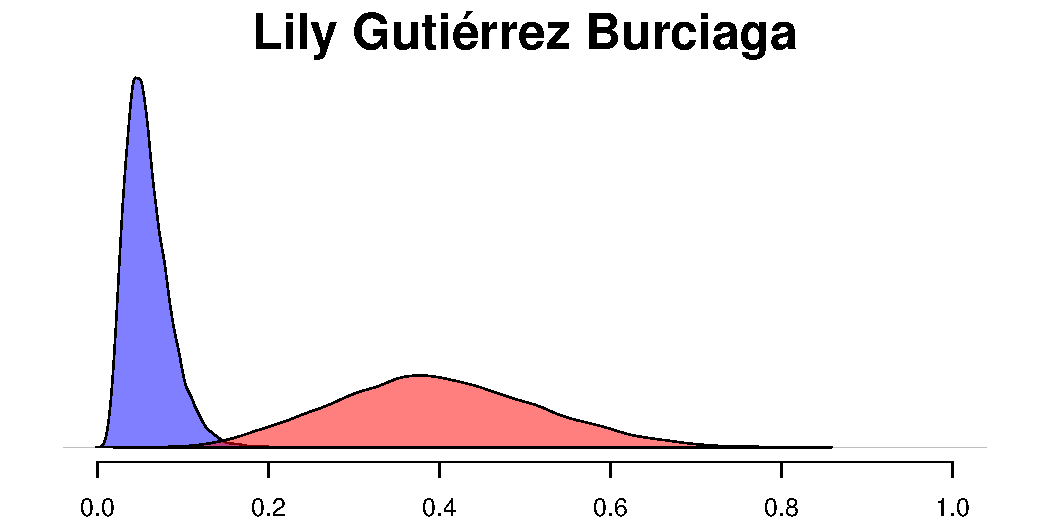
\includegraphics[width=.45\columnwidth]{../graphs/prReconoce2.pdf} &
    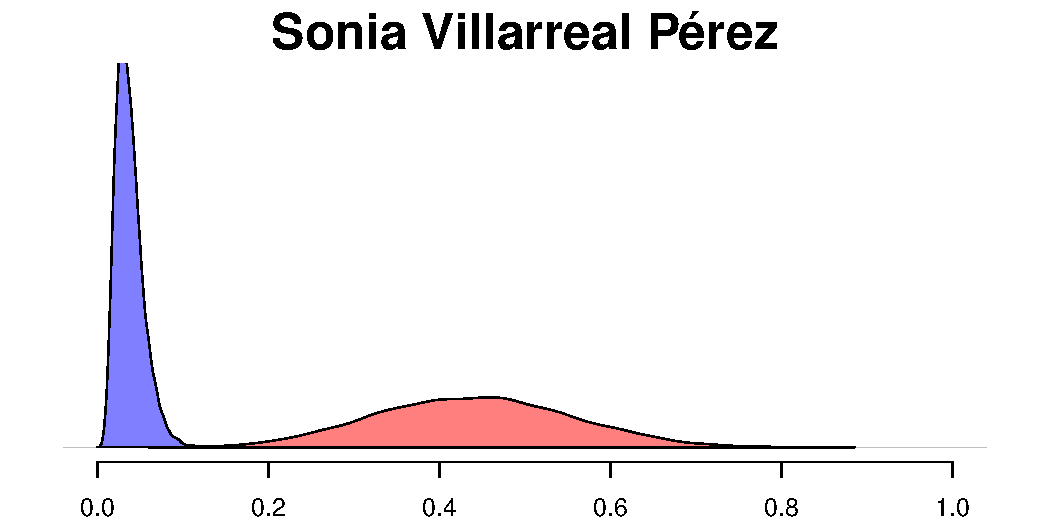
\includegraphics[width=.45\columnwidth]{../graphs/prReconoce5.pdf} \\
    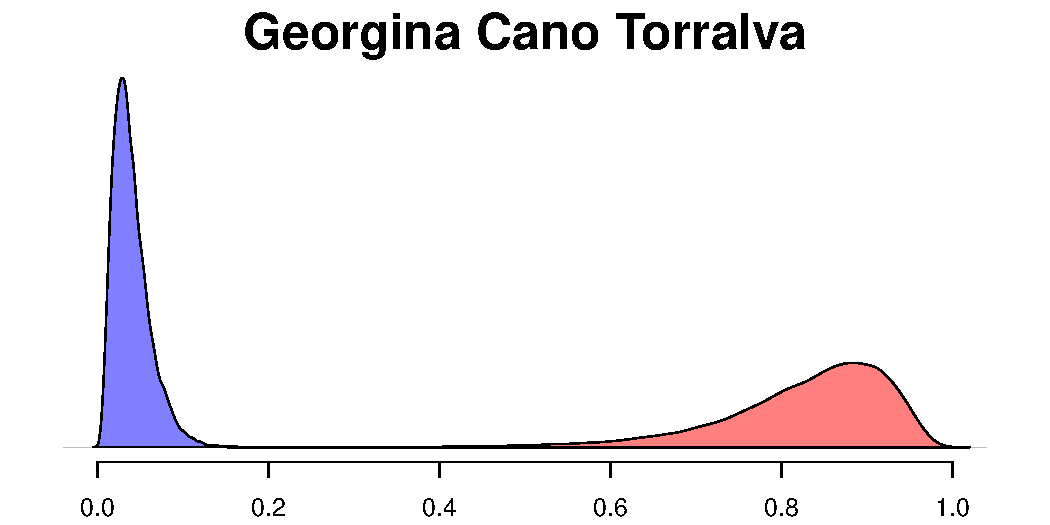
\includegraphics[width=.45\columnwidth]{../graphs/prReconoce3.pdf} &
    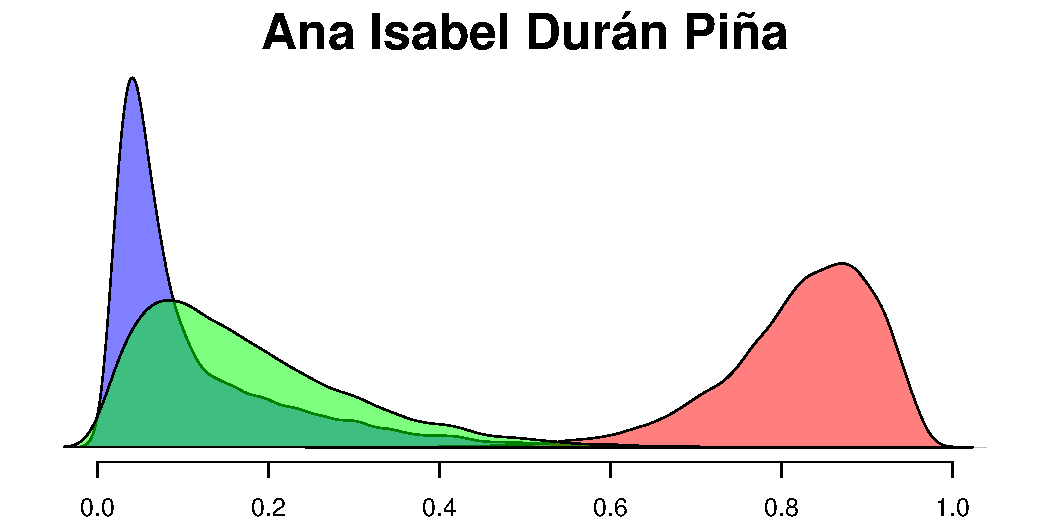
\includegraphics[width=.45\columnwidth]{../graphs/prReconoce4.pdf} \\
  \end{tabular}
~ \\ ~ \\ ~ \\
%\definecolor{MidnightBlue}{rgb}{0.1, 0.1, 0.44}
\definecolor{MidnightBlue}{rgb}{0.48, 0.41, 0.93}
\definecolor{LimeGreen}{rgb}{0.2, 0.8, 0.2}
\definecolor{Salmon}{rgb}{1.0, 0.55, 0.41}
\medskip
\begin{tabular}{|rc|}
  \hline \multicolumn{2}{|c|}{\textbf{Hypotheses}:} \\
  incumbency & \textcolor{MidnightBlue}{$n$} $<$ \textcolor{LimeGreen}{$l$} $=$ \textcolor{Salmon}{$r$} \\
  campaign   & \textcolor{MidnightBlue}{$n$} $=$ \textcolor{LimeGreen}{$l$} $<$ \textcolor{Salmon}{$r$} \\ \hline
\end{tabular}
\medskip
\caption{The probability of name recognition (x-axis). Simulations generated with Bayesian estimations of regression models. The violet density is for respondents in area $n$, the green (when applicable) for respondents in area $l$, and the pink for respondents in area $r$. Incumbency leads to expect the purple to lie to the left, the pink to the right, the green between them, with clear gaps between them. All other controls held constant to represent a PAN-identifier with a smartphone, who said the incumbent has delivered but is uninterested in politics.}\label{f:sims}
\end{figure}

% \bibliographystyle{apsrInitials}
% \bibliography{/home/eric/Dropbox/mydocs/magar}

\end{document}
